\documentclass{article}
\usepackage[backend=bibtex]{biblatex}
\usepackage[utf8]{inputenc}
\usepackage[german]{babel}
\usepackage{caption}
\usepackage[skip=0.5ex]{subcaption}
\usepackage[left=3cm,right=3cm,top=2cm,bottom=2cm]{geometry}
\usepackage[pdfborder={0 0 0}]{hyperref} % Kein Rahmen um die 

\usepackage{color}
\usepackage{xcolor}
\usepackage{listings}
\definecolor{commentgreen}{rgb}{0.15,0.42,0.2}
\definecolor{codegray}{rgb}{0.5,0.5,0.5}
\definecolor{stringred}{rgb}{0.6,0.12,0.12}
\definecolor{functionblue}{rgb}{0,0,1}
\definecolor{backcolor}{rgb}{0.95,0.95,0.92}
\definecolor{linkcolor}{rgb}{0, 0.05, 0.3}

\usepackage{hyperref}
\hypersetup{
    colorlinks=true,
    linkcolor=linkcolor,
    filecolor=magenta,      
    urlcolor=cyan,
    pdftitle={DB2 Summary},
    pdfpagemode=FullScreen,
    }

\usepackage{parskip} % do not indent first lines
\usepackage{bookmark}
\usepackage{booktabs}
\usepackage{textcomp}
\usepackage{array}
\usepackage{graphicx}
\usepackage{amsmath}

\usepackage{color}
\usepackage{xcolor}
\usepackage{listings}

\lstset{language=Java,
  commentstyle=\color{commentgreen},
  keywordstyle=\color{functionblue},
  numberstyle=\tiny\color{codegray},
  stringstyle=\color{stringred},
  basicstyle=\ttfamily\fontsize{14}{14},
  breakatwhitespace=false,         
  breaklines=true,                 
  captionpos=b,                    
  keepspaces=true,                 
  numbers=left,                    
  numbersep=5pt,                  
  showspaces=false,                
  showstringspaces=false,
  showtabs=false,                  
  tabsize=2
}

\newcommand{\quotes}[1]{''#1''}

\graphicspath{ {./images/} }

\begin{document}
\title{Summary\\Datenbanken 2 - SoSe 2021}
\author{Jonas Weßner}
\maketitle
\tableofcontents
\newpage				% Neue Seite nach TOC

\section{Einführung}

\subsection{Impedance Mismatch}
Impedance Mismatch bezeichnet eine Gruppe von typischen Schwierigkeiten, mit denen sich auseinander gesetzt werden muss, wenn eine Anwendung, die in einer objektorientierten Programmiersprache geschrieben ist, mit einer relationalen Datenbank zusammenarbeiten soll.\\
Objektorientierte Sprachen benutzen dabei vor allem folgende Konzepte, die nicht in relationalen Datenbanken vorkommen:
\begin{itemize}
    \item Inheritance
    \item Komposition - Listen und komplexe Objekte können Attribute eines Objekts sein
    \item Objektidentität durch Referenzgleichheit oder überladenen Equality-Operator
\end{itemize}

Relationale Datenbanken nutzen vor allem folgende Konzepte, die nicht in der Objektorientierung vorkommen:
\begin{itemize}
    \item Identität eines Tupels mit Primärschlüssel
    \item Fremdschlüssel mit FK-Contraints
    \item Atomarität von Spaltenwerten (1. Normalform) mit nur primitiven Datentypen
\end{itemize}

\subsection{Object-Relational Mapping - ORM}
Object-relational mapping bezeichnet die Gruppe von Lösungsansätzen, die sich mit dem Konvertieren von Daten zwischen der relationalen und objektorientierten Welt befasst. Dabei versuchen sie dementsprechend mit dem Impedance Mismatch möglichst gut umzugehen. Das Ziel ist dabei, dass dieses mapping weitestgehend automatisiert von Statten geht und die Vorteile beider "Welten" hervorgehoben werden.\\
Es existieren mehrere Ansätze, die man i.d.R. in Top-Down oder Bottom-Up einordnen kann.\\
Bei \textbf{Top-Down}-Ansätzen konvertiert ein OR-Mapper die Klassen eines Anwendungsprogramms in ein Datenbankschema. Dementsprechend kümmert es sich um die Erstellung und den Zugriff auf die Datenbank. Ein Beispiel für einen Top-Down-Ansatz ist z.B. die JPA (Java Persistence API), die in diesem Dokument noch näher betrachtet wird.\\
Bei \textbf{Bottom-Up}-Ansätzen wird mittels eines Reverse-Engeneering-Tools aus einem existierenden Datenbankschema versucht ein objektorientiertes Modell zu extrahieren. Dieser Ansatz wird in diesem Dokument nicht weiter verfolgt.\\
\\
Darüber hinaus befassen sich ORM-Tools/Frameworks i.d.R. auch mit \textbf{Transaktionsmanagement} und \textbf{Caching}. Dies sind Aufgaben, die über die Lösung des Impedance Mismatch hinaus gehen.
\section{Java Persistence API - JPA}
\subsection{Was ist die JPA?}
Die Java Persistence API ist eine Spezifizierung für eine API, die von verschiedenen ORM-Frameworks implementiert wird. Dabei umfasst sie folgende Bereiche:
\begin{itemize}
    \item Die API für Annotationen, die im java.persistence package definiert ist
    \item Die Java Persistence Query Language \textbf{JPQL}
    \item Metadaten über Objekte und Relationen
\end{itemize}
Die Referenzimplementierungen der JPA 2 (aktuell) ist EclipseLink. Weitere Implementierungen sind z.B. Hibernate, Oracle TopLinkEssentials, Apache OpenJPA und Bea Kodo. Verschiedene Implementierungen der JPA können sich in manchen Punkten auch in ihrer Funktionalität unterscheiden (so wie auch z.B. SQL sich von DBMS zu DBMS unterscheiden kann).\\
Das Prinzip ist so aufgebaut, dass Java Klassen mit Metadaten angereichert werden, sodass der OR-Mapper diese Klassen in ein relationales Schema überführen und in die Datenbank schreiben kann. Früher wurden XML-Dateien verwendet, um diese Meta-Daten zu definieren. Heute werden die Metadaten durch Java-Annotations definiert (deutlich einfacher, kürzer und übersichtlicher).

\subsection{Begrifflichkeiten}
\subsubsection*{Persistenzkontext}
Der Persistenzkontext ist die Menge aller Objekte von Entity-Klassen, die der dem EntityManager zugeordneten PU zugeordnet sind, und von einem Entity Manager verwaltet werden. Jede Veränderung eines Objektes im Persistenzkontext wirkt sich beim nächsten Commit auf die darunterliegende Datenbank aus. Jedes Objekt besitzt maximal eine relationale Repräsentation in der DB (falls ein Objekt gerade erst in den Persistenzkontext aufgenommen wurde, besitzt es keine Repräsentation bis zum nächsten Commit, mehr dazu später).

\subsubsection*{Persistence Unit (PU)}
Persistence Units werden als XML angegeben und definieren eine Mapping-Konfiguration für eine Menge von Klassen (die dementsprechend mit @Entity gekennzeichnet sein müssen).\\
Die Konfigurationen können zahlreiche Dinge enthalten, wie:
\begin{itemize}
    \item URL, Benutzername, Password für den DB Zugriff
    \item Table Generation Strategie
    \item Logging Konfiguration
          \begin{itemize}
              \item ''drop-and-create'': Beim Start alle Tabellen löschen, die benutzt werden sollen und dann diese neu anlegen. Somit also nur auf leeren Tabellen arbeiten
              \item ''create'': Falls eine Tabelle noch nicht existiert wird sie angelegt, andernfalls weiterverwendet
              \item ''none'': Die DB wird nicht verändert. D.h. die Tabellen müssen schon zu Beginn existieren, ansonsten gäbe es einen Fehler
          \end{itemize}
\end{itemize}

Ein EntityManagerFactory kann genau einer PU zugeordnet werden. Mit ihr können dann mehrere EntityManager erzeugt werden, die auch dieser PU zugeordnet sind.

\subsection{Basic Annotations}
Annotationen definieren in Klassen die Metadaten, die der OR-Mapper benötigt, um sie in die Datenbank mappen zu können. Solche Klassen, für die eine Datenbankrepräsentation erstellt werden kann, nennt man auch Entity-Klassen.\\
Einige einfache Annotationen sind:
\begin{itemize}
    \item \textbf{@Entity}: Entity Klasse
    \item \textbf{@Id}: Primary Key der zugehörigen Entity in der DB
    \item \textbf{@GeneratedValue(strategy = ''...'', generator = ''...'')}: Ein automatisch vom DBMS generierter Wert. Der Wert sollte beim Aufruf von manager.persist noch nicht gesetzt sein und wird dann von der DB generiert. Optional kann noch angegeben werden mit welcher Strategie dieser Wert generiert werden soll und welchen Namen die Spalte für das Zählen dieses Generator-Wertes bekommen soll.
    \item \textbf{@Temporal(TemporalType.XXX)}: Gibt für Datumstypen an, welche Art von Datum in der DB dafür benutzt werden soll. In Java ist z.B. die Klasse Date sehr verbreitet, in SQL gibt es allerdings mehrere verschiedene Datentypen für Zeiten.
    \item \textbf{OrderBy(''spalte'')}: Gibt für Collections an, dass beim Laden aus der DB der Inhalt der Collection nach dem Primary Key Attribut sortiert oder optional nach einem bestimmten anderen Attribut sortiert geladen werden soll.
    \item \textbf{@OrderColumn(name = ''new\_col\_name'')}: Wird für Collections benutzt. Fügt der Entity ein zusätzliches Attribut hinzu, das dazu benutzt wird, die Reihenfolge der Daten in der Collection beim schreiben in die Datenbank zu speichern. Wird das Objekt dann aus der DB geladen, so ist die Reihenfolge der Objekte in der Collection wieder so, wie bei dem Objekt, das persistiert wurde. Wird nicht diese Annotation oder die OrderBy Annotation angewendet, so ist die Reihenfolge der Elemente einer Collection beim Laden aus der DB willkürlich.
\end{itemize}
Im nächsten Unterkapitel werden wir die Annotationen \textbf{@OneToMany}, \textbf{@ManyToOne}, \textbf{@ManyToMany}, \textbf{@JoinTable} und \textbf{@ElementCollection} etwas genauer betrachten. Es gibt auch noch zahlreiche andere Annotationen, in deren Dokumentation man sich mithilfe der hier gezeigten Beispiele gut einarbeiten können sollte.

\subsection{Beziehungen zwischen Entity-Klassen}

\subsubsection{1:n OneToMany Beziehungen}
In Java können unidirektionale Beziehungen und bidirektionale Beziehungen dargestellt werden.\\
Eine \textbf{unidirektionale Beziehung} entsteht typischerweise, wenn eine Klasse (umschließende Klasse) als Attribut eine Collection vom Typ einer anderen Klasse (umschlossene Klasse) enthält. So enthält ein Objekt dieser umschließenden Klasse (One) keine bis viele Objekte der umschlossenen Klasse (Many). Wenn man nun ein Objekt der umschließenden Klasse hat, kann man mittels durchsuchen der Collection alle Objekte der umschlossenen Klasse finden, die dem Objekt der umschließenden Klasse zugeordnet sind. Allerdings ist das andersherum nicht möglich, da die umschlossene Klasse keine Referenz auf die umschließende Klasse enthält. Daher ist auch die umschlossene Klasse nicht von der umschließenden Klasse abhängig.\\
Eine \textbf{bidirektionale Beziehung} entsteht, wenn der Sachverhalt einer unidirektionalen Beziehung gegeben ist und zusätzlich die umschlossene Klasse als Attribut auch eine Referenz auf ein Objekt der umschließenden Klasse enthält. Auf diese Weise kann auch nur mit einem Objekt der umschlossenen Klasse herausfinden, welchem Objekt der umschließenden Klasse es zugeordnet ist. Diese Herangehensweise bietet mehr Flexibilität aber birgt auch die Gefahr von Inkonsistenzen. So ist es möglich einem Objekt in der umschlossenen Klasse eine Referenz auf ein Objekt der umschließenden Klasse zu speichern, dem es tatsächlich von der anderen Seite aus betrachtet nicht zugewiesen ist (also wenn es nicht Teil der Collection des Objektes der umschlossenen Klasse ist).\\
\\
In JPA werden grundsätzlich beide Möglichkeiten unterstützt. Wenn wir jedoch betrachten, wie solche Beziehungen in einer Relationalen DB dargestellt werden, fallen 2 Dinge auf:
\begin{enumerate}
    \item Es gibt nur unidirektionale 1:n Beziehungen
    \item Die Beziehungen werden so dargestellt, dass die Tabelle der 1-Seite ein Attribut hat, dass FK der n-Seite ist. Auf diese Weise wird jedem Element der 1-Seite tatsächlich genau 0-1 Elemente der n-Seite zugeordnet. Allerdings ist das genau andersherum, wie wir es in OO-Programmiersprachen üblicherweise machen. Das liegt daran, dass wir in der Programmierung mit Collections arbeiten, aber in DB das Prinzip der Atomarität haben, dass Listentypen als Attribute verbietet.
\end{enumerate}
Aus \textbf{1.} folgt, dass beim schreiben von Objekten mit bidirektionalen Beziehungen nur eine der Beziehungen dargestellt wird.\\
Aus \textbf{2.} folgt, dass wir uns überlegen müssen, wie zwischen den beiden Darstellungen konvertiert wird.\\
\\
Im unteren Beispielbild wollen wir das obere ER-Modell mithilfe von Java Entity-Klassen generieren. Dazu können wir eine bidirektionale Beziehung implementieren, bei der jede Kategorie eine Collection an Artikeln hat und jeder Artikel eine Referenz auf die ihm zugeordnete Kategorie enthält. Da wir in der DB nur eine unidirektionale Beziehung darstellen wollen und können, müssen wir mithilfe von Annotationen angeben, welche Seite für die erstellung der Beziehung benutzt werden soll. Dabei enthält das Referenzattribut der Kategorie die Annotation @OneToMany und das des Artikels ManyToOne. Da wir wollen, dass die 1-Seite, also die Artikel, in der DB ein Attribut haben, das auf die Kategorie verweist, geben wir in der Kategorie \textit{mappedBy = ''kategorie''} an. Dies teilt JPA mit, dass dieses Attribut schon durch ein Attribut in einer anderen Klasse, das den Namen \textit{kategorie} trägt, dargestellt wird und somit in dieser Klasse ignoriert werden kann. Somit wird also beim generieren der DB die Collection (meineArtikel) nicht mit in das Schema aufgenommen, das Attribut der 1-Seite (kategorie) wird allerdings aufgenommen und auch als FK gekennzeichnet.


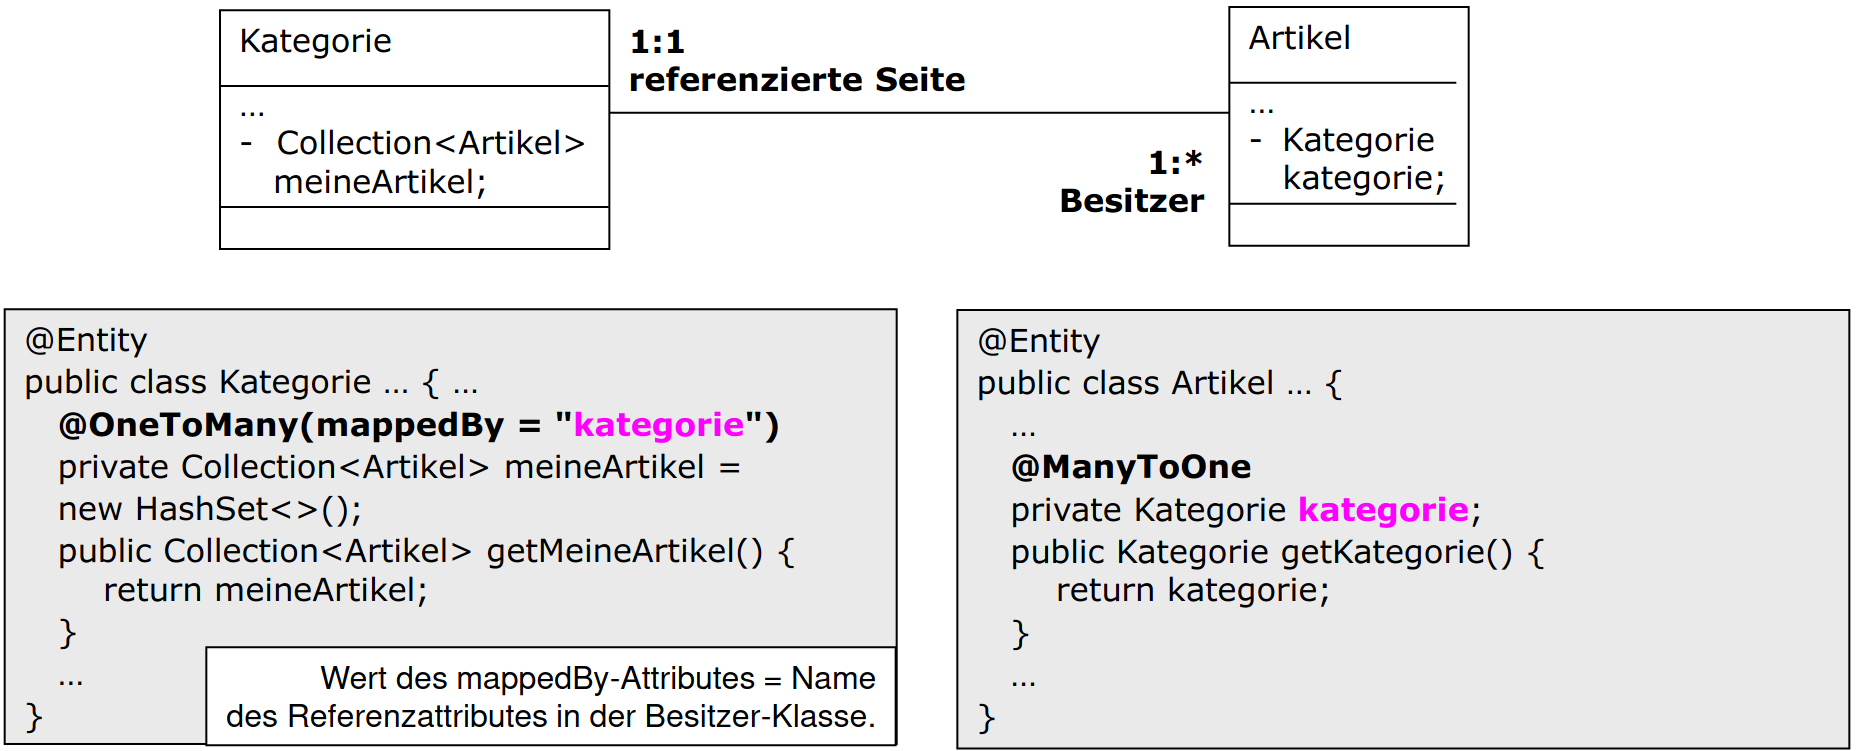
\includegraphics[width=500px]{JPAOneToMany.png}

1-n Beziehungen in Java direkt in 1-n Beziehungen in der DB zu mappen ist zwar laut der Spezifikation auch möglich, aber nicht empfehlenswert, da die Implementierung nicht korrekt ist. Im Beispiel würde dann bei unserem Klassendiagramm die Klasse Kategorie nur die \textit{@OneToMany} Annotation ohne den Zusatz von \textit{mappedBy} bekommen. Bei der Klasse Artikel würde dann die Referenz auf die Kategorie und damit auch die Annotation fehlen.\\
Das Problem hierbei ist, dass daraus dann in der DB tatsächlich keine 1:n Beziehung, sondern eine n:m Beziehung generiert werden würde. D.h. es würde eine Zwischentabelle erzeugt werden, die Kombinationen von Primärschlüsseln der beiden Tabellen als Fremdschlüssel speichert.


\subsubsection{n:m ManyToMany Beziehungen}
In Java können n:m Beziehungen, wie auch 1:n Beziehungen (siehe vorheriges Kapitel), sowohl unidirektional, als auch bidirektional dargestellt werden.\\
\textbf{Unidirektionale n:m Beziehung} würde bedeuten, dass wir genau wie bei einer unidirektionalen 1:n Beziehung eine umschließende Klasse haben, die eine Collection von Referenzen auf eine umschlossene Klasse enthält. Nur hier würden wir erlauben, dass wir eine Referenz auf ein und das selbe Objekt der umschlossenen Klasse in den Collections mehrerer verschiedener Objekte der umschließenden Klasse enthalten haben. Das heißt designtechnisch ist das Java Klassendiagramm genau wie für eine 1:n Beziehung, der Unterschied ist nur der Umgang damit.\\
\textbf{Bidirektionale n:m Beziehung} würde bedeuten, dass beide Klassen eine Collection allen mit Referenzen auf Objekte der anderen Klasse haben, denen sie zugeordnet sind.\\
\\

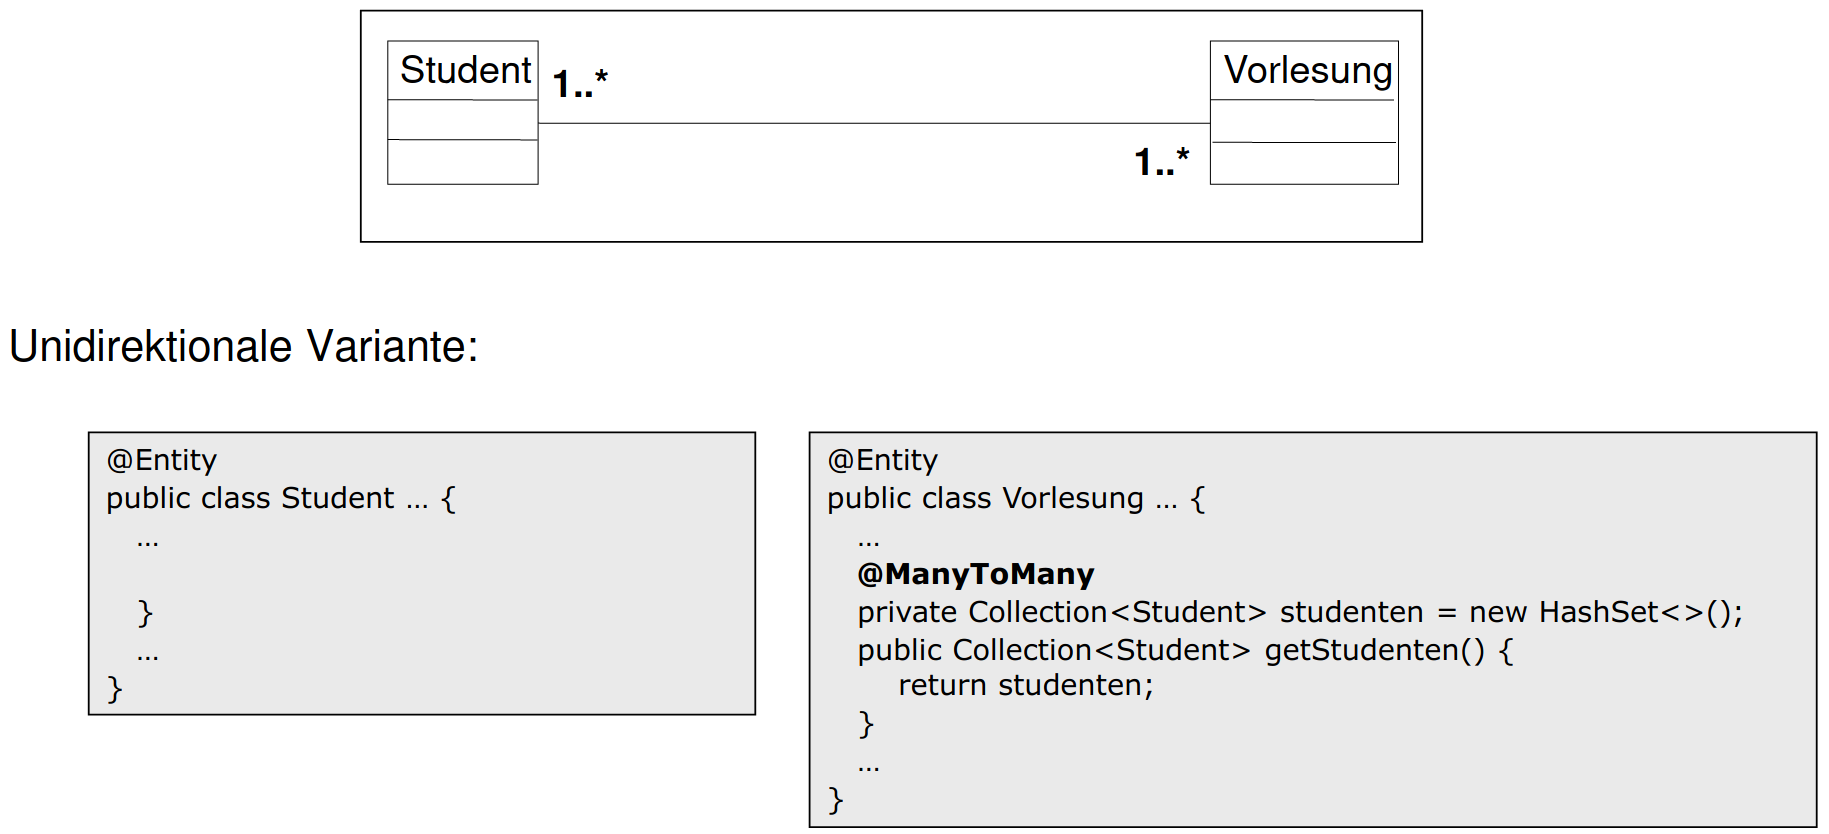
\includegraphics[width=400px]{JPAManyToManyUnidirectional.png}

Der unidirektionale Fall ist sehr einfach umgesetzt. Hier kann einfach die Annotation \textit{@ManyToMany} bei der Collection benutzt werden. Zusätzlich kann optional noch die Annotation \textit{@JoinTable(name=''table\_name'')} benutzt werden, um zu bestimmen, wie die Zwischentabelle in der DB, die die Beziehung abbildet, benannt werden soll. Es gibt auch noch andere Annotationen, mit denen auch die Namen der Attribute personalisiert werden können, auf die hier nicht weiter eingegangen wird.

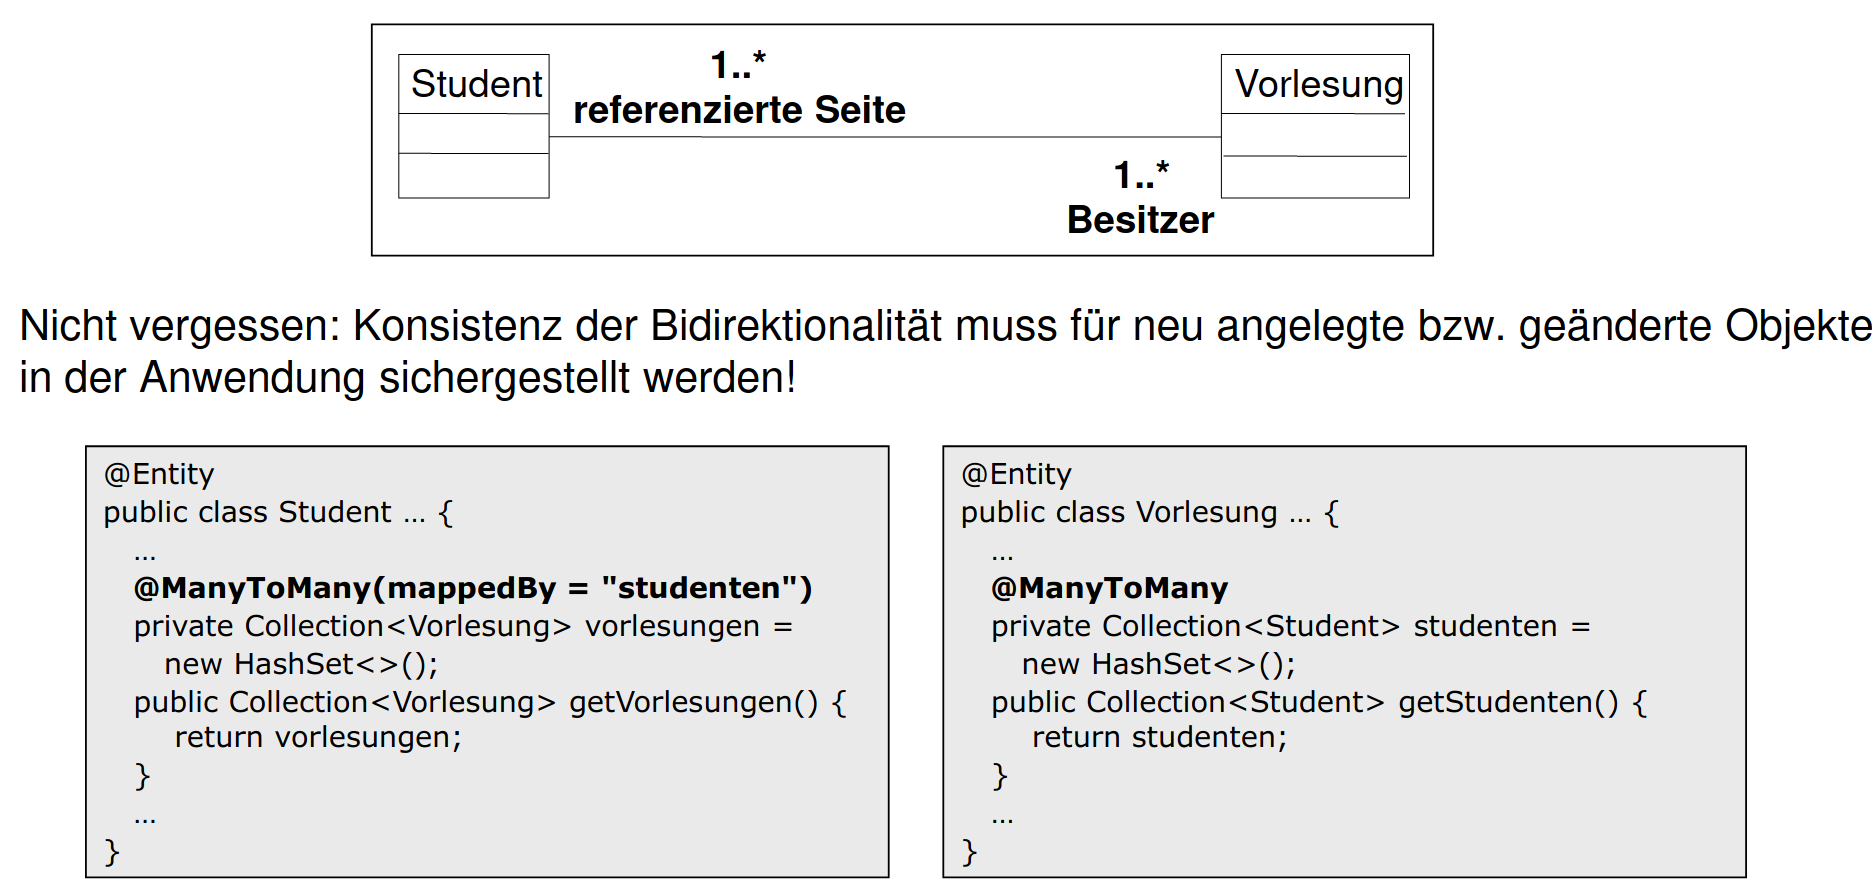
\includegraphics[width=400px]{JPAManyToManyBidirectional.png}

Bei der bidirektionalen Variante haben wir die Information über die Beziehung zwischen den Entity-Klassen doppelt gespeichert (und hoffentlich Konsistent). Deshalb müssen wir hier, wie auch bei der bidirektionalen 1:n Beziehung, auf einer Seite beim Referenzattribut mittels \textit{mappedBy = ''attribut\_name''} anzeigen, dass diese Beziehung bereits durch ein anderes Attribut mit dem Namen attribut\_name dargestellt wird. Das heißt JPA wird das so annotierte Attribut ignorieren. Dadurch entsteht für JPA eine unidirektionale Beziehung, die wie oben erklärt abgebildet wird. Für den Programmierer bleibt jedoch die Flexibilität der bidirektionalen Beziehung bestehen.


\subsubsection{Kompositionen komplexer Typen und Collections}
Zuvor haben wir nur primitive Datentypen als Komposition darstellen können. Für andere Datentypen wurde mit den Annotationen \textit{@OneToMany} eine Assoziation erstellt. Um auch Kompositionen von Komplexen Typen darstellen zu können müssen wir den Typ, der eingebettet sein soll, statt mit \textit{@Entity} mit \textit{@Embeddable} annotieren. Wird dieser Typ dann in einer umschließenden Klasse als Komposition benutzt, so muss dieses Attribut als \textit{@Embedded} annotiert werden.\\
Der Unterschied zu einer Assoziation einer mit \textit{@Entity} annotierten Klasse ist dabei, dass das Hinzufügen und Löschen von Objekten der umschließenden Klasse zur umschlossenen Klasse kaskadieren, so wie wir es in OO-Programmiersprachen von Kompositionen gewöhnt sind.\\

Im Fall von einem einzigen \textit{@Embedded}-Attribut werden alle Attribute der eingebetteten Klasse in der Datenbank als Attribute der umschließenden Klasse angelegt. Im Falle einer \textit{@EmbeddedCollection} wird eine separate Relation benötigt.

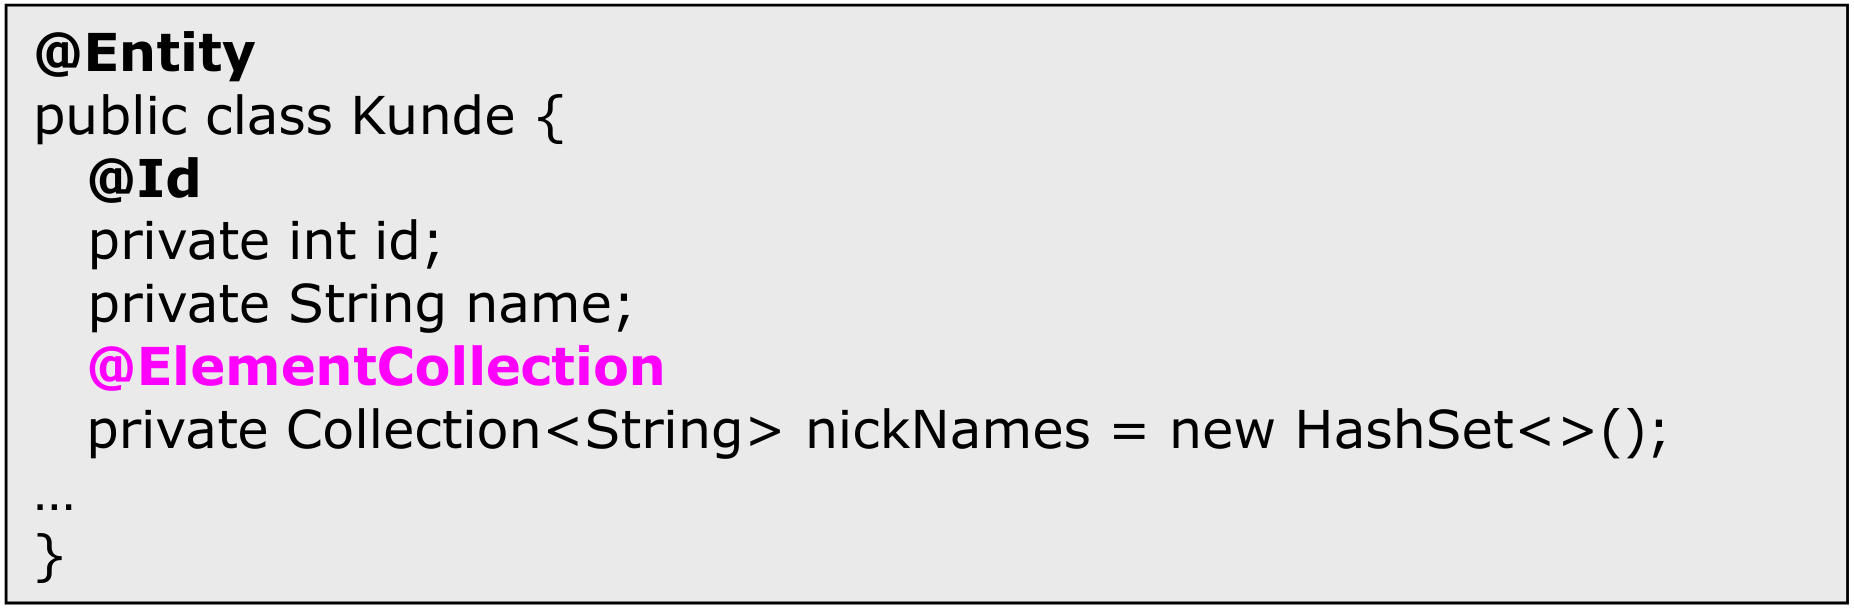
\includegraphics[width=300px]{JPAElementCollection.png}

\textbf{Collections} können als \textit{@EmbeddedCollection} annotiert werden, um eine Komposition einer Collection herbeizuführen. Dabei muss der Typ der Collection ein primitiver Typ, den in in der DB auch gibt, oder eine mit \textit{@Embeddable} annotierte Klasse sein. Tatsächlich wird in der DB sehr wohl eine weitere Tabelle angelegt, um das zu bewerkstelligen, aber diese wird so abstrahiert, dass die Collection in der Java-Anwendung als Komposition betrachtet werden kann. Dabei ist zu beachten, dass mit \textit{@Embeddable} annotierte Klassen keine \textit{@Id}-Annotation benötigen.

\subsubsection{Inheritance}
die in OO-Programmiersprachen und im Relationenmodell bekannte Inheritance (Vererbung) gibt es so in relationalen Datenbanken nicht. Doch man kann Vererbung auf 3 verschiedene Weisen abbilden lassen. Um JPA mitzuteilen, welche Strategie angewendet werden soll, wird in der Elternklasse die Annotation \textit{\textbf{@Inheritance(strategy = InheritanceType.XXXX)}} benutzt. Die verschiedenen Strategien werden hier kurz erläutert:
\begin{itemize}
    \item \textbf{InheritanceType.JOINED}: Für jede Klasse, auch für Superklassen, wird eine Tabelle erstellt. Wenn alle Instanzen der einer abstrakten Klasse benötigt werden, also z.B. alle Bücher (Audiobooks, Taschenbücher...) muss nur die Tabelle für die abstrakte Klasse durchsucht werden. Allerdings werden selbst für den Zugriff auf Daten einer abgeleiteten Klasse JOINS benötigt, weil einige Attribute aus dem Table, der der Superklasse zugeordnet ist, geholt werden müssen.
    \item \textbf{InheritanceType.SINGLE\_TABLE}: Für alle Klassen der Vererbunghierarchie wird nur ein gemeinsamer Table angelegt. Zeilen haben dann NULL Werte an den Attributen, die es in der Klasse, der sie entstammen, nicht gab. Der Vorteil ist der schnelle Zugriff ohne JOINS. Der Nachteil ist die Verschwendung von Speicherplatz für die NULL Werte.
    \item \textbf{InheritanceType.TABLE\_PER\_CLASS}: Erstellt für jede konkrete Klasse eine Tabelle. Attribute von abstrakten Superklassen werden in den Tabellen der abgeleiteten Klassen eingefügt. Wenn man alle Datensätze, die zu Subtypen einer abstrakten Klasse gehören, muss man nun mehrere Tabellen, nämlich so viele, wie es abgeleitete Klassen gibt, durchsuchen. Diese Strategie ist in JPA optional spezifiziert und wird nicht von allen Frameworks implementiert.

\end{itemize}

\subsection{Funktionsweise des Frameworks}
\subsubsection{Entity-Lifecycle}
\vspace{5px}
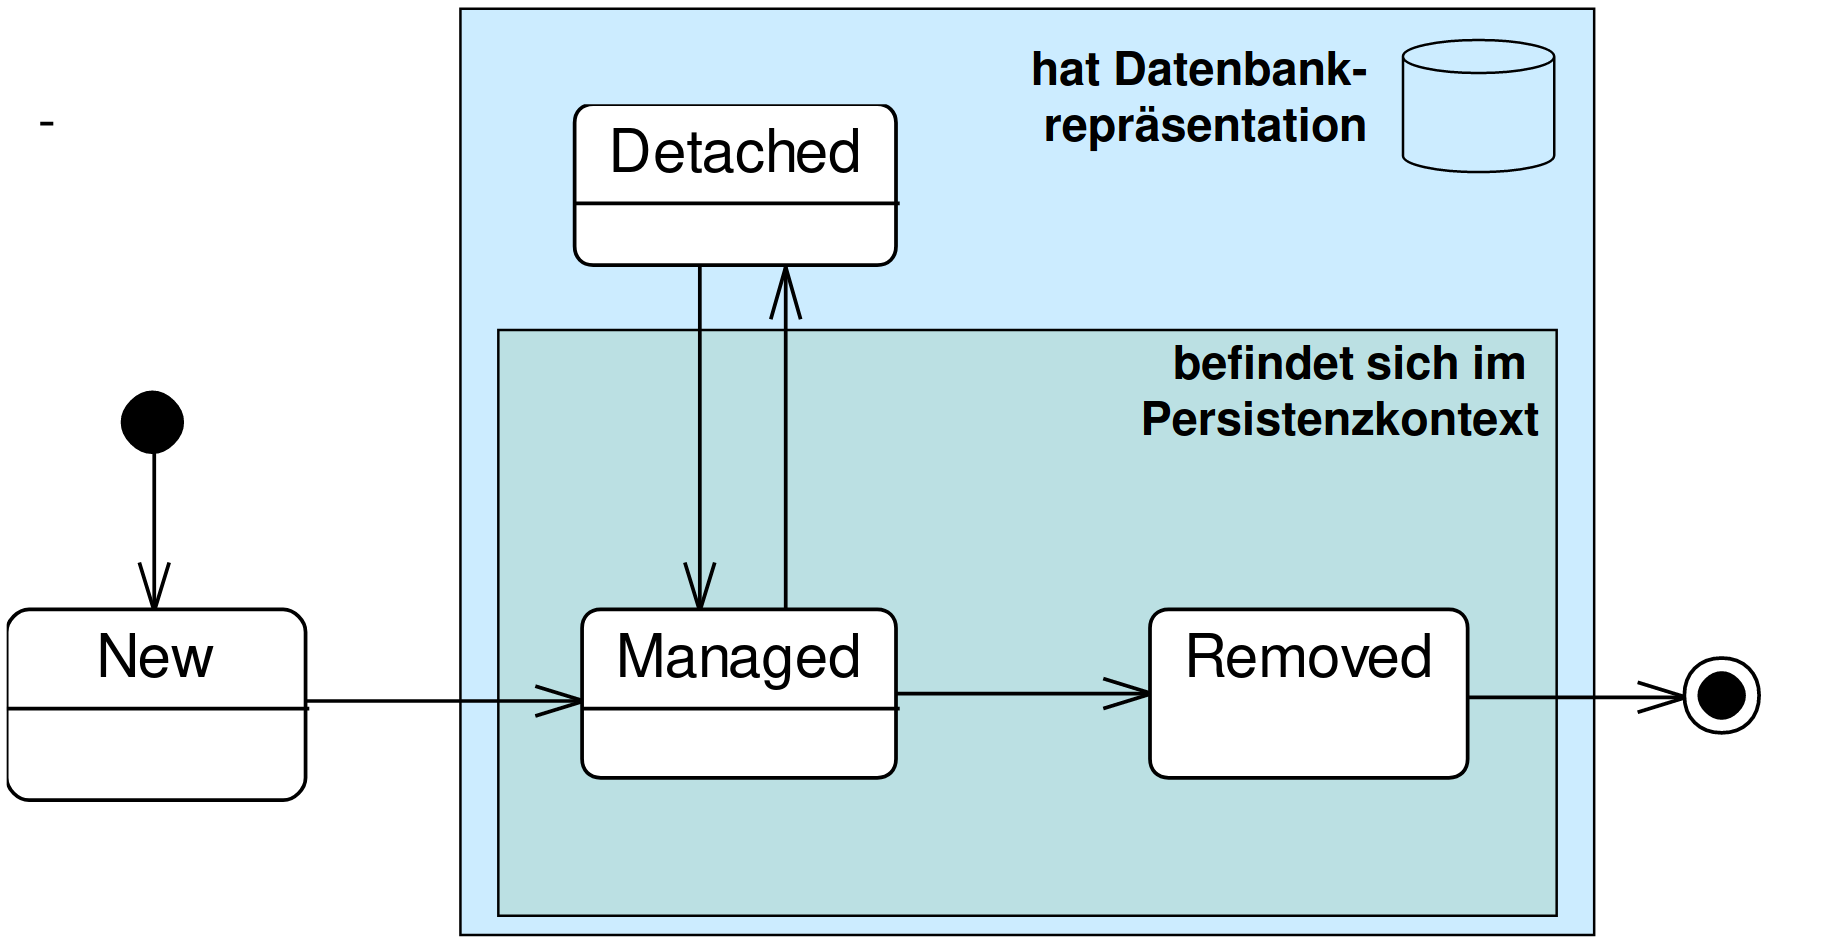
\includegraphics[width=400px]{JPAEntityLifecycle.png}

Eine Instanz einer Entity-Klasse kann sich in 4 verschiedenen Zuständen befinden:
\begin{itemize}
    \item \textbf{New}: Wenn ein Objekt erzeugt wird, ist es zunächst nicht im Persistenzkontext. Es ist in dieser Zeit also nur ein einfaches, vom OR-Framework unabhängiges Objekt.
    \item \textbf{Managed}: Das Objekt befindet sich im Persistenzkontext. Es hat 0-1 relationale Repräsentation in der DB (keine falls es gerade erst dem Persistenzkontext hinzugefügt wurde und die Änderung noch nicht commitet wurde). Änderungen an dem Objekt werden beim nächsten Commit mit der Datenbank synchronisiert.
    \item \textbf{Detached}: Das Objekt hat eine Repräsentation in der Datenbank, befindet sich aber nicht im Persistenzkontext, wird also zurzeit nicht mehr vom EntityManager verwaltet. Es ist also wieder unabhängig vom ER-Framework.
    \item \textbf{Removed}: Das Objekt soll aus der Datenbank gelöscht werden. Beim nächsten Commit wird die Repräsentation dann aus der Datenbank gelöscht und es wird aus dem Persistenzkontext genommen.
\end{itemize}

Um Objekte zwischen den verschiedenen Zuständen zu bewegen, gibt es Methoden der EntityManager-Class. Einige sollen im Folgenden vorgestellt werden:
\begin{itemize}
    \item \lstinline{void persist(Object obj)}: Nimmt ein Objekt in den Persistenzkontext auf.
    \item \lstinline{T find(Class<T> entityClass, Object primaryKey)}: Sucht eine Entity anhand ihres Primary Keys im Persistenzkontext. Falls es nicht gefunden wird, sucht es das Objekt in der Datenbank. Falls gefunden, wird das entsprechende Objekt zurückgegeben, andernfalls \textbf{null}.
    \item \lstinline{T getReference(Class<T> entityClass, Object obj)}: wie find(), nur das eventuell bloß eine noch im Cache vorhandene Version geladen wird, die eventuell dirty ist.
    \item \lstinline{boolean contains(Object obj)}: Gibt zurück, ob ein Objekt im Persistenzkontext ist
    \item \lstinline{void refresh(Object obj)}: Aktualisiert das Objekt im Persistenzkontext durch Nachladen seiner relationalen Repräsentation in der DB. D.h. falls die Daten in der DB inzwischen durch andere parallelle Prozesse geändert wurden, kann der Persistenzkontext aktualisiert werden.
    \item \lstinline{void remove(Object obj}: Schiebt eine Entity in den Zustand removed (siehe oben).
    \item \lstinline{void flush()}: Erzwingt die Abwärtssynchronisation von Hauptspeicher nach DB schon vor dem Commit.
    \item \lstinline{void detach(T entity)}: Schiebt ein Objekt in den Zustand detached, es befindet sich dann nicht mehr im Persistenzkontext.
    \item \lstinline{T merge(T entity)}: Fügt eine Copy eines detached Objektes wieder in den Persistenzkontext ein und gibt eine Referenz auf das eingefügte Objekts zurück.
    \item \lstinline{ void clear()}: Detached alle Objekte.
\end{itemize}

\subsubsection{Transaktionen und Sessions}
\begin{itemize}
    \item Beim Erzeugen eines EntityManagers über EntityManagerFactory.getEntityManager() wird eine DB-Session für diesen EntityManager eröffnet.
    \item Beim Aufruf von EntityManager.close() wird die DB-Session dieses EntityManagers geschlossen.
    \item Beim Aufruf von EntityManager.getTransaction().begin() wird eine Transaktion innerhalb der Session des EntityManagers gestartet.
    \item Beim Aufruf von EntityManager.getTransaction().commit() wird diese Transaktion beendet.
\end{itemize}

\subsubsection{Transitive Persistenz}
Normalerweise beziehen sich die Funktionen persist(), merge(), remove() ,refresh() und detach() nur auf das Objekt, mit dem sie aufgerufen werden. Also nicht für Objekte, die als Attribute mit @ManyToOne, @OneToMany, @ManyToMany, @OneToOne enthalten sind. Für diese müssen die Funktionen gesondert aufgerufen werden. Um die Funktionsaufrufe zu kaskadieren und damit auch für die referenzierten Objekte auszuführen, kann man noch den Zusatz cascade = CascadeType.XXXX hinzufügen.\\
Bsp.:\\
\textbf{@OneToMany( cascade = CascadeType.PERSIST)}

\subsubsection{Callback Methoden}
Methoden einer Entity-Class können mit bestimmten Annotationen als Callback Methoden für Aufrufe von bestimmte Methodenaufrufe der EntityManager Klasse eingetragen werden. Der Effekt ist ähnlich dem von Triggern:
\begin{itemize}
    \item @PrePersist
    \item @PostPersist
    \item @PostLoad
    \item @PreUpdate
    \item @PostUpdate
    \item @PreRemove
    \item @PostRemove
\end{itemize}
\section{Datenbankabfragen - JPA Query Interface}

Das JPA Query Interface ist eine Programmierschnittstelle, die Klassen zur Abfrage von Daten, die mittels JPA persistiert wurden, abzufragen. Die JPA bietet 3 verschiedene Ansätze, die alle ihre Vor- und Nachteile mit sich bringen:

\subsection{JPQL}
Die JPQL (Java Persistence Query Language) ist eine Datenbanksprache, die syntaktisch sehr stark an SQL angelegt ist. Hierbei werden Anfragen auf Basis von Klassen gestellt. Der OR-Mapper findet dann heraus wie die Klassen relational gespeichert sind, erzeugt die entsprechenden SQL-Queries aus dem JPQL-Query und mappt die Ergebnisse der SQL-Queries direkt in Objekte der abgefragten Klasse. Die JPQL ist vom konkreten darunterliegenden DBMS unabhängig, wodurch Portierbarkeit gewährleistet wird. Allerdings können deshalb auch DBMS-spezifische Features nicht genutzt werden.\\
Die Methoden zur Erstellung von Queries ist mit folgenden Methoden möglich:
\begin{itemize}
    \item \lstinline{EntityManager.createQuery(String jpql);} Erstellen einer dynamischen Query, die zur Laufzeit kompiliert wird.
    \item \lstinline{EntityManager.createNamedQuery(String queryName);} Abrufen einer statischen Query, die zur Kompilierzeit des Java-Programms kompiliert wird und typsicher ist. Diese Query muss zuvor in einer Annotation definiert sein.
\end{itemize}

\subsubsection{Dynamische Queries}

Eine dynamische Query wird durch den Aufruf von \\
\lstinline{EntityManager.createQuery(String jpql);}\\
erzeugt. Dabei ist das Argument eine Abfrage in der Sprache JPQL. Ein Beispiel wäre:\\

\lstinline{em.createQuery("select e from Employee e");}\\

Diese Query wird in der DB alle relationalen Repräsentationen von Objekten der Klasse \lstinline{Employee} suchen, daraus die entsprechenden Objekte erzeugen und diese zurückliefern.\\
Es ist auch möglich \textbf{nur einzelne Attribute einer Klasse} zu erhalten. In diesem Fall ist das Ergebnis dann eine Liste von Arrays, bei der jedes Array Element ein Attribut enthält:\\

\lstinline{em.createQuery("select e.id, e.name from Employee e");}\\

Diese Query liefert also eine Liste von Arrays mit 2 Elementen.\\
Es ist auch möglich \textbf{parametrisierte Queries} zu erzeugen. Diese enthalten Parameter, die mit einem Doppelpunkt gekennzeichnet werden. Diese Parameter können dann z.B. mit Nutzereingaben gefüllt werden. Dabei werden alle für JPQL relevanten Schlüsselwörter u.Ä. escaped, sodass eine SQL injection verhindert werden kann:\\


\begin{lstlisting}
    var query em.createQuery("select e from Employee e where e.name = :name");
    query.setParameter("name", "Smith");
\end{lstlisting}

\textbf{Ausführen von Queries:}\\

Sobald eine Query erzeugt wurde, kann sie ausgeführt werden. Dies geschieht mit einem der folgenden Aufrufe:
\begin{itemize}
    \item \lstinline{query.getResultList();} Gibt eine Liste von Ergebnisobjekten zurück, über die iteriert werden kann
    \item \lstinline{query.getSingleResult();} Gibt genau ein Ergebnisobjekt zurück. Wirft eine Exception, falls mehr als ein Objekt oder kein Objekt gefunden wird. Kann benutzt werden, wenn mit Sicherheit (z.B. bei Abfrage nach einem Objekt mit einem bestimmten PK) nur ein Objekt zurückgegeben wird.
    \item \lstinline{query.executeUpdate();} Kann für Massen Updates und Deletes verwendet werden.
\end{itemize}

\textbf{Beispiel für Ausführen von Queries:}\\

\begin{lstlisting}
    List resultList = em.createQuery("select e from Employee e").getResultList();
    
    for(Iterator i = resultList.iterator(); i.hasNext();){
        Employee e = (Employee) i.next();
        System.out.println(e.toString());
    }
\end{lstlisting}

\subsubsection{(Statische) Named Queries}

Im Gegensatz zu normalen Queries, bei denen das JPQL zur Laufzeit interpretiert wird und damit Syntaxfehler zur Laufzeit möglich sind, können Named Queries bereits zur Kompilierzeit des Java Programms gecheckt werden.\\
Dazu wird eine Query mit einer Annotation direkt an einer Klasse definiert. Die Query kann dann im Code über ihren Namen gefunden werden.\\
Die Vorteile von Named Queries sind:
\begin{itemize}
    \item Syntaxüberprüfung zur Kompilierzeit
    \item Performance, wegen Vorkompilierung
    \item Keine Code Replikation bei häufig verwendeten Queries
\end{itemize}

\textbf{Beispiel für Named Queries:}\\
Definition als Annotation:

\begin{lstlisting}
    @Entity
    @NamedQueries({
        @NamedQuery(name="Employee.findAll",
            query="select e from Employee e"),
        @NamedQuery(name="Employee.findByName",
            query="select e from Employee e where e.name=:name")}) 
    public class Employee implements Serializable{ ... }
\end{lstlisting}

Abrufen der Query:

\begin{lstlisting}
    List resultList = em.createNamedQuery("Employee.findAll").getResultList();
    ...
    List resultList = em.createNamedQuery("Employee.findByName").setParameter("name", "Smith").getResultList(); 
\end{lstlisting}

\subsubsection{Implizite JOINs}

Da wir bei der Verwendung von JPQL eine Abstraktion benutzen, welche die wahren ausgeführten SQL-Queries vor uns verbirgt, kann es vorkommen, dass eine JPQL Anfrage implizite JOINS erzeugt. Da JOINS Performance kosten, sollten wir uns dieser Tatsache bewusst sein. Implizite Joins entstehen immer dann, wenn ein Attribut einer Klasse zurückgeliefert werden soll, das selbst wieder eine Entity-Class ist. Denn diese zwei Klassen werden von JPA in verschiedenen Relationen gespeichert.\\
Beispiel, bei dem sowohl \lstinline{Order} als auch \lstinline{Customer} Entity-Classes sind:

\begin{lstlisting}
    List resultList = em.createQuery("select o.customer from Order o").getResultList();
\end{lstlisting}

\subsubsection{Explizite JOINs}

Explizite JOINs sind in JPQL auch möglich. Diese sind aber nur nötig, wenn 2 Klassen gejoint werden sollen, die in keiner Klassenrelation stehen.

\subsection{JPA Native SQL Queries}

Mit der Methode \lstinline{EntityManager.createNativeQuery(String sql)} kann eine native SQL Query erzeugt werden. Der Vorteil davon ist, dass auch DBMS-Spezifische Features genutzt werden können. Der große Nachteil ist, dass der ORM uns dann nicht die Arbeit mit der relationalen DB abnimmt und wir somit die Stärken von JPA nicht nutzen können.

\subsection{JPA Criteria API}

In der JPA Criteria API wird zusätzlich zum Klassenmodell noch ein statisches Metamodell erstellt, das für eine bestimmte Persistence Unit bestimmt ist. Die Queries werden dann objektorientiert basierend auf diem Metamodell formuliert.

\textbf{Vorteile:}

\begin{itemize}
    \item Typsicherheit und Syntax zur Kompilierzeit überprüft
\end{itemize}

\textbf{Nachteile:}

\begin{itemize}
    \item Komplexe Queries werden sehr unübersichtlich
    \item Umstieg von SQL gewöhnungsbedürftig
\end{itemize}
\section{Performance Optimierung beim OR-Mapping}

\subsection{Transaktionsmanagement}
\subsubsection{Funktionsweise von Sessions und Transactions}

Wenn wir mit JPA arbeiten, gilt im Bezug auf Sessions und Transaktions das Folgende:

\begin{itemize}
    \item Der Lebenszyklus einer Instanz der EntityManager-Class ist Äquivalent zu einer DB-Session. In dieser kann es mehrere Transactions geben.
    \item Die Dauer zwischen den Aufrufen von Transaction.begin() und Transaction.commit() ist die Dauer einer Transaction. Änderungen werden erst beim Aufruf von Transaction.commit() in die DB geschrieben. Damit ist gewährleistet, dass alle Operationen einer Transaction ausgeführt werden oder garkeine.
\end{itemize}

Auf \textbf{Datenbankebene} wird beim Aufteten eines Fehlers eine uncommitted Transaction zurückgerollt (rollback).\\
Tritt auf \textbf{Anwendungsebene} allerdings eine Exception auf, so kann das DBMS nichts davon mitbekommen. In diesen Fällen sollte die Transaction explizit zurückgerollt werden. Das kann dann ungefähr so aussehen:

\begin{lstlisting}
    EntityManager em = emf.createEntityManager(); // start session
    EntityTransaction t;
    try{
        t = em.getTransaction();
        t.begin();

        // (...)

        t.commit();
    } catch(RuntimeException e){
        if(t != null && t.isActive()){
            t.rollback();
        }
        throw e; // optionally rethrow exception to handle by caller
    } finally {
        em.close(); // close session
    }
\end{lstlisting}

\subsubsection{Best Practices für Transactionsmanagement}
Dem Entwickler ist freigestellt wie er Transactions und Sessions einsetzen möchte. Es ergeben sich folgende Möglichkeiten mit ihren Vor- und Nachteilen:

\begin{enumerate}
    \item \textbf{Session per Request-Pattern:} Jede Transaction in einer eigenen Session durchführen, d.h. immer eine neue Instanz der EntityManager-Class benutzen.\\
          \textbf{Vorteile:}
          \begin{itemize}
              \item Beim Start jeder Transaction ist der Persistenzkontext frisch und konsistent mit dem Zustand der DB
          \end{itemize}
          \textbf{Nachteile:}
          \begin{itemize}
              \item Beim schließen des EntityManager-Objekts gehen alle Java-Objekte, die sich im Persistenzkontext befinden, vom Zustand persisted in den Zustand detached über. Soll mit diesen Objekten in einer weiteren Transaktion (und also auch weiteren Session) weitergearbeitet werden, so müssen sie dem Persistenzkontext des neuen EntityManager-Objekts wieder explizit zugefügt werden. Dies geschieht über den Aufruf von merge()
              \item Erzeugen vieler einzelner Sessions ist weniger performant (erst bei vielen Sessions ausschlaggebend)
          \end{itemize}
    \item \textbf{Transaction per Request:} Jede Transaction in der gleichen Session durchführen, dh. alle Transactions über das selbe EntityManager-Objekt abschließen.\\
          \textbf{Vorteile:}
          \begin{itemize}
              \item Java-Objekte, die im Persistenzkontext des EntityManager-Objekts sind, können über mehrere Transactions weiter verwendet werden.
          \end{itemize}
          \textbf{Nachteile:}
          \begin{itemize}
              \item Mit zunehmender Zeit, die eine Session aktiv ist steigt die Chance, dass Java-Objekte, die im Persistenzkontext sind, von anderen konkurrierenden DB-Zugriffen manipuliert wurden und sich also auf DB-Ebene verändert haben. Es empfiehlt sich eine explizite Synchronisation mit EntityManager.refresh() durchzuführen.
          \end{itemize}
    \item Ein \textbf{Mittelweg} der beiden oberen Herangehensweisen.
\end{enumerate}

Wir sehen also, dass die Länge der Sessions, vor allem auch mit Bezug auf die Wahrscheinlichkeit von konkurrierenden Zugriffen, abgewägt werden muss.

\subsection{Caching}

\subsubsection{First-Level-Cache}
Der First-Level-Cache ist immer aktiv und an ein Entity-Manager-Objekt gebunden. Er gilt also für genau eine DB-Session. Die Aufgabe des First-Level-Cache ist es die Anzahl der SQL-Statements, die an die DB gesendet werden zu minimieren. Beispielsweise werden mehrere UPDATEs auf dem selben Objekt innerhalb einer Transaction zu einem einzigen UPDATE Statement zusammengefasst, welches zum Zeitpunkt des Commits übertragen wird. Ebenso werden Objekte, die bereits von der DB in den Persistenzkontext geladen wurden vom First-Level-Cache gespeichert und bei einer erneuten Anfrage zurückgegeben anstatt sie mit einer weiteren Query erneut zu laden.

\subsubsection{Second-Level-Cache}
Der Second-Level-Cache ist ein Cache, der an eine EntityManagerFactory und damit an eine DB-Connection gebunden ist. Er muss vom Entwickler explizit in der Persistence-Unit des Projekts aktiviert werden:
\begin{lstlisting}
    <property name="javax.persistence.sharedCache.mode" value="XXX" />
\end{lstlisting}

Mögliche Werte für diese Property sind:
\begin{itemize}
    \item ALL
    \item NONE
    \item ENABLE\_SELECTIVE
    \item DISABLE\_SELECTIVE
\end{itemize}

Im Second-Level-Cache werden die Ergebnisse von Queries sessionübergreifend gespeichert. Bei der Abfrage von Daten wird zuerst der First- dann der Second-Level-Cache und erst dann die DB durchsucht, um die Daten zu finden.

\subsection{Ladestrategien}

\subsubsection{Eager Loading vs. Lazy Loading}

Nehmen wir nun zur Veranschaulichung an, dass wir zwei Java-Klassen haben, Car und Engine:

\begin{lstlisting}
@Entity
public class Car {
    public String licensePlate;
    private Engine engine;
    // (...)
}
@Entity
public class Engine {
    // (...)
}
\end{lstlisting}

Wenn wir nun ein Car-Objekt mit JPQL aus der DB abfragen, müssen wir uns bewusst sein, dass dadurch ein impliziter Join benötigt wird. Car und Engine liegen also in unterschiedlichen DB-Tabellen und müssen gejoint werden, damit ein vollständiges Objekt der Klasse Car zurückgegeben werden kann. Wenn Engine jetzt wiederum Datenelemente einer anderen Entity hätte (Komposition), dann würde sich diese Kette fortsetzen und wir müssten auf DB-Ebene weitere Joins durchführen. Um auf dieses Verhalten Einfluss zu nehmen gibt es 2 Herangehensweisen zwischen denen sich entschieden werden kann:\\

\textbf{Eager Loading:}\\
Mit Eager Loading bezeichnen wir eine Ladestrategie, bei der wir angeforderte Objekte einmalig und vollständig von der DB laden. Das bedeutet, dass wir im Auto-Beispiel auch das Objekt der Engine-Klasse laden, wenn wir das Auto laden. Bei sehr verschachtelten Strukturen oder Kompositionen von Collections kann diese Herangehensweise dazu führen, dass sehr viele Daten geladen werden. Falls dann in Wirklichkeit gar nicht alle Informationen benötigt werden (im Beispiel etwa nur die licensePlate und nicht die Engine ausgelesen wird), dann haben wir großen unnötigen Mehraufwand gehabt, der uns Performance kostet. Falls tatsächlich alle Daten des Objektes benötigt werden, muss dagegen nichts mehr nachgeladen werden und alles liegt schon bei dem Ergebnis einer einzigen (wenn auch JOIN-behafteten) Query vor.

\textbf{Lazy Loading:}\\
Mit Lazy Loading bezeichnen wir eine Ladestrategie, bei der wir Attribute, die vom Typ anderer Entity-Klassen sind, nicht mitladen, sondern nur sogenannte Proxy-Objekte laden. Sobald auf ein Proxy-Objekt zugegriffen wird, führt JPA dann im Hintergrund eine Query aus, die das tatsächliche Objekt nachlädt.\\
Im Auto-Beispiel würde also beim Abfragen eines Autos nur ein Proxy-Objekt der Engine geladen werden. Falls dann auf die Referenz zugegriffen wird, lädt JPA dynamisch die Daten für das tatsächliche Engine-Objekt. Auf diese Weise kann man sich eine große Menge der Datenübertragung sparen, falls tatsächlich nie auf das Attribut zugegriffen werden sollte. Falls jedoch doch auf das Attribut zugegriffen wird, hat man Performance verloren, weil man zwei separate Queries an das DBMS senden musste.\\
In diesem Zusammenhang ist der Begriff \textbf{n+1-Problem} wichtig. Das n+1-Problem besagt, dass wir im Falle von Lazy Loading im schlechtesten Fall n+1 Datenbankzugriffe haben, wobei n die Anzahl der lazy geladenen Attribute ist. Wir benötigen nämlich n Zugriffe für die n Attribute und noch einen Zugriff zu Beginn für das Objekt der umschließenden Klasse.\\

Wir sehen also, dass Eager Loading geschickter ist, wenn man bereits im Vorhinein weiß, dass man ein Attribut tatsächlich benutzen wird. Andersherum ist Lazy Loading geschickter wenn man ein Attribut eher nicht oder auf jeden Fall nicht benutzen wird.

\subsubsection{Syntax von Eager- und Lazy-Loading in JPA}

Um die Loading Strategy für ein Attribut festzulegen, annotieren wir dieses Attribut wie folgt mit FetchType.LAZY oder FetchType.EAGER:

\begin{lstlisting}
    @OneToMany(fetch = FetchType.XXX)
    @ManyToOne(fetch = FetchType.XXX)
    @ManyToMany(fetch = FetchType.XXX)
    @Basic(fetch = FetchType.XXX) // for 1-1 compositions
\end{lstlisting}

Die Default Werte sind wie folgt:

\begin{itemize}
    \item \textbf{XxxToMany:} LAZY
    \item \textbf{XxxToOne} und \textbf{Basic:} EAGER
\end{itemize}

Falls ein Attribut mit LAZY annotiert ist, aber in einer bestimmten Query doch mit der Strategie EAGER geladen werden soll, kann in der Query der sogenannte FETCH JOIN benutzt werden:

\begin{lstlisting}
    SELECT c from Customer c JOIN FETCH c.articles
\end{lstlisting}

In der oberen Query wird mittels JOIN FETCH erzwungen, dass das Attribut articles der Klasse Customer direkt mitgeladen wird, so als ob das Attribut mit fetch = FetchType.EAGER annotiert wäre.

\subsection{Lesen großer Datenmengen}

Paging und Scrolling sind Methoden, die genutzt werden können, um mit Anfragen zu arbeiten, die potentiell sehr große Datenmengen zurückgeben.

\subsubsection{Paging}
Paging bezeichnet das Verfahren bei dem nur eine Teilmenge der Ergebnismenge der Query zurückgegeben wird. Dabei gibt man den Startindex und die Anzahl der Zeilen an. Paging ist also sinnvoll, um die Datenmenge zu begrenzen. Paging ist allerdings nicht sinnvoll, wenn man eine große Datenmenge stückweise verarbeiten möchte. Dann müsste man sich nämlich den Index merken bis zu dem man in der vorherigen Iteration gelesen hat und außerdem sicherstellen, dass sich die Indices der einzelnen Zeilen zwischen Queries nicht verändern. Für solche Szenarien ist dann \hyperref[sec:scrolling]{Scrolling} besser geeignet.\\
In JPA wird Paging benutzt, indem man die folgenden Instanzmethoden der Klasse Query benutzt:

\begin{lstlisting}
    Query.setFirstResult(int);
    Query.setMaxResults(int);
\end{lstlisting}

Paging wird auch auf DB-Ebene unterstützt, sieht syntaktisch jedoch je nach SQL-Dialekt unterschiedlich aus. Deshalb ist es vorteilhaft, dass JPA die Übersetzung in den SQL-Dialekt des konkreten genutzten DBMS übernimmt.

\subsubsection{Scrolling}
\label{sec:scrolling}

Scrolling bezeichnet ein Verfahren bei dem eine Art Iterator benutzt wird, um über eine Ergebnisrelation zu iterieren. Scrolling wird nicht im JPA-Standard, wohl aber von JDBC und Hibernate unterstützt.\\
In \textbf{JDBC} geschiet dies über den Aufruf von der Methode next() auf dem ResultSet-Objekt:
\begin{lstlisting}
    Statement stmt = con.createStatement();
    ResultSet rs = stmt.executeQuery("Select * from MyPlayers");
    while(rs.next()){
         // (...)
    }
\end{lstlisting}

\subsection{Manipulieren großer Datenmengen}

\subsubsection{Bulk-Operationen}
\label{sec:bulk-operations}
Als Bulk-Operationen bezeichnet man Statements, die mehrere Zeilen beeinflussen. Der Vorteil von Bulk-Operationen im Vergleich zu einzelnen Statements ist, dass nur ein Statement an das DBMS gesendet werden muss, die Datenübertragung also sehr gering ist.\\
In \textbf{SQL} kennen wir diesbezüglich das UPDATE und das DELETE Statement. Diese Statements beeinflussen alle Zeilen der Tabelle. Es können aber auch bestimmte Zeilen mit einem WHERE herausgefiltert werden.\\
Auch in \textbf{JPA} gibt es diese Operationen.

\begin{lstlisting}[language=SQL]
    UPDATE ClassName c
    SET c.attribute = newValue
    WHERE c.attribute = oldValue;

    DELETE ClassName c
    WHERE c.attribute = value;
\end{lstlisting}

Der Unterschied zu SQL ist hier aber, dass wir nicht mit Tabellen, sondern mit Klassen arbeiten. Das bedeutet, dass auch Vererbungshierarchien und Kompositionen beachtet werden.

\subsubsection{Batch-Operationen}
Als Batch-Operationen bezeichnet man das Senden von mehreren Statements an das DBMS in einem "`Rutsch''. Das ist sinnvoll, wenn viele Zeilen verändert werden sollen, aber die Logik zu komplex ist, um die Änderung mit einer einzigen \hyperref[sec:bulk-operations]{Bulk-Operation} durchzuführen.\\
Batch-Operationen werden von \textbf{JDBC} seit Version 2.0 unterstützt. Dafür werden die Instanzmethoden der Statement-Class genutzt, um einzelne Batches einem Statement hinzuzufügen:

\begin{lstlisting}
Statement stmt = conn.createStatement();
conn.setAutoCommit(false);

stmt.addBatch("INSERT INTO ...");
stmt.addBatch("DELETE FROM ...");
stmt.addBatch("UPDATE ...");

int[] count = stmt.executeBatch();

// explicitly commit changes
conn.commit();
\end{lstlisting}

Batch Writing ist im JPA-Standard nicht definiert, wird allerdings von manchen Implementierungen, z.B. der bei uns im Praktikum verwendeten Eclipse Link, trotzdem unterstützt. Dazu müssen zwei Einträge in der Persistence Unit vorgenommen werden, die , welcher Service für Batch-Operationen benutzt werden soll und wie viele Operationen in einem Batch zusammengefasst werden sollen:
\begin{lstlisting}[language=XML]
    <propertyname="eclipselink.jdbc.batch-writing" value="JDBC"/>
    <propertyname="eclipselink.jdbc.batch-writing.size" value="1000"/>
\end{lstlisting}
\section{Performance Optimierung auf DBMS-Ebene}

In diesem Kapitel soll es darum gehen, wie das DBMS Queries möglichst performant ausführt und wie wir diese Ausführung analysieren und beeinflussen können.

\subsection{Puffermanagement}

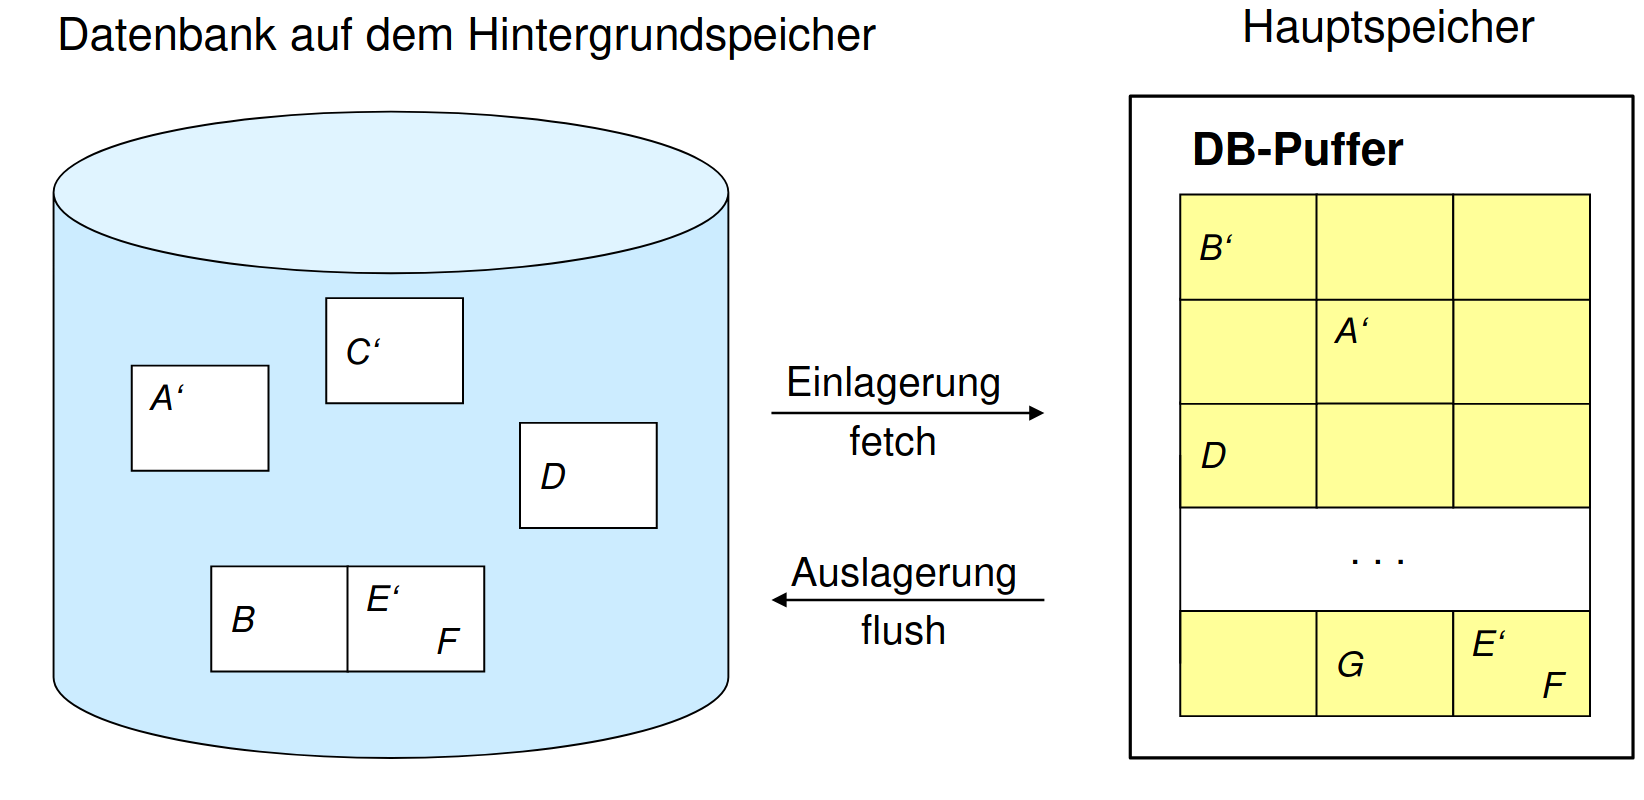
\includegraphics[height=150px]{DB-Puffer.png}

Das DBMS möchte möglichst schnell auf abgefragte Daten zugreifen können. Um dies zu tun, lädt es einige Daten von der langsameren Festplatte in den schnelleren Hauptspecher. Dies macht natürlich besonders viel Sinn, wenn die dort liegenden Daten häufig abgefragt werden. Folglich ist im DBMS komplexe Logik vorhanden, die versucht möglichst effiziente \textbf{Caching-Strategien} umzusetzen. \\

Das DBMS führt auch Statistiken über den Zugriff. Das bedeutet, dass konkret auch die Anzahl der Zugriffe und die Anzahl der Cache-Hits getrackt wird, sodass die Effizienz des Caching Verfahrens analysiert werden kann. Die Statistiken sind in DBMS-spezifischen internen Tabellen abgelegt, die auch abgefragt werden können.

\subsection{Zugriffsarten}

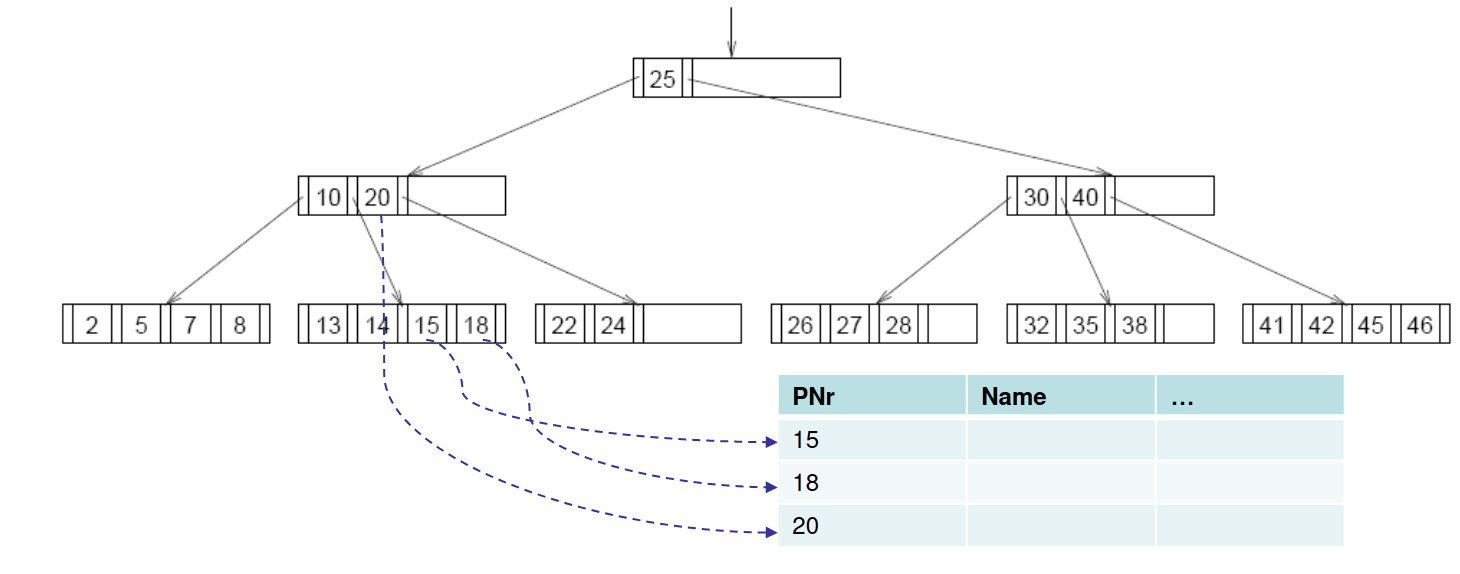
\includegraphics[height=150px]{B-Tree.png}

\textbf{B-Tree}, balanced tree, ist eine Datenstruktur, die zur effizienten Suche benutzt werden kann. In jedem Knoten werden Elemente sortiert abgelegt. Kind-Knoten werden so gelinkt, dass sie jeweils nur Elemente enthalten, die in der Sortierung zwischen zwei Elementen des Eltern-Knoten liegen. Jeder Knoten hat eine maximale Anzahl an Elementen, die er enthalten kann, bevor Elemente in ein neues Kind ausgelagert werden. Innerhalb der Knoten kann eine lineare Suche durchgeführt werden, die aufgrund der niedrigen Anzahl der Elemente trotzdem performant ist. Durch die verschiedenen Stufen des Baumes kann der Bereich, in welchem sich das gesuchte Element befindet, schnell eingegrenzt werden, sodass nur ein Bruchteil des gesamten Baumes mit linearer Suche durchlaufen werden muss. \\
Der B-Tree eignet sich offensichtlich auch gut für Bereichsanfragen, also Anfragen bei denen alle Elemente in einem bestimmten Bereich, der sich auf das Sortierkriterium bezieht, abgefragt werden.

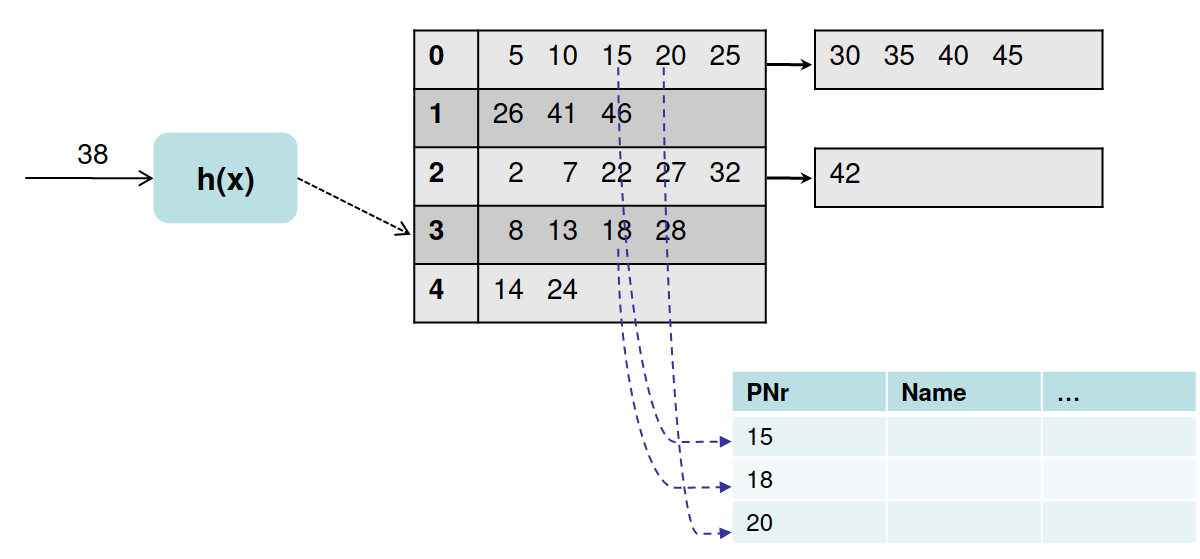
\includegraphics[height=150px]{Hash-Function.png}

\textbf{Hash-Funktionen} sind Funktionen, die eine gegebenenfalls unendlich große Menge von Eingabeelementen auf einen endlich großen Wertebereich abbilden. Die Hash-Funktion soll sehr effizient berechenbar sein, z.B. modulo. Wir können also für ein gegebenes Element den Hash-Wert berechnen. Wenn wir die Hash-Werte und die Ihnen zugeordneten vorhandenen Elemente nach dem Hash-Wert sortiert abspeichern, können wir zu einem Hash-Wert schnell alle zugehörigen Elemente finden. Wenn unsere Hash-Funktion die Elemente möglichst gleichmäßig auf die verschiedenen Werte abbildet, ist gewährleistet, dass die Anzahl der Elemente mit dem selben Hash-Wert sehr gering ist. Deshalb können wir effizient die lineare Suche anwenden, um unser gesuchtes Element in den Elementen mit dem selben Hash-Wert zu suchen. \\
Hash-Funktionen sind sehr performant für das Einfügen und Abrufen einzelner Elemente, da nur einmal die Hash-Funktion angewendet werden muss (im Gegensatz zum B-Tree, bei dem man mehrere Stufen durchlaufen muss). Allerdings sind sie für Bereichsabfragen schlecht geeignet, da die Hash-Werte von Elementen in keinem Zusammenhang zu ihrem Bereich (innerhalb einer Sortierung) stehen und somit der Hash-Wert für jedes einzelne Element berechnet werden muss.

\subsection{Optimizer-Strategien}

Der Optimizer ist die Komponente des DBMS, die bestimmt, auf welche Weise ein Query ausgeführt werden soll. Dazu bestimmt er zunächst alle sinnvollen Ausführungspläne für die Query. Diese Ausführungspläne zeichnen sich durch die Art und Reihenfolge der Operationen aus, sowie durch die dafür verwendeten Technologien (z.B. B-Tree vs. Hash). Dann entscheidet er sich für den aus seiner Sicht besten Ausführungsplan. Die Wahl, die der Optimizer trifft, hängt im Wesentlichen auch von den ihm zur Verfügung stehenden Mittel ab, also z.B. den Indexen. Der Optimizer führt auch Statistiken über die Distribution der Inhalte in den Tabellen, sodass er aufgrund dieser Information Rückschlüsse über die Effizienz von bestimmten Verfahren ziehen kann. Z.B. kann es sein, dass die gleiche Query mit den gleichen Indexen bei verschiedenen Datenbeständen unterschiedlich ausgeführt wird. Konkret ist nämlich das Benutzen eines Hash-Indexes nur dann performanter als eine lineare Suche, wenn auch so viele Daten vorliegen, dass die Daten auf verschiedene DB-Seiten verteilt werden. So wird der Optimizer wahrscheinlich beim Abfragen von Daten aus einer Tabelle mit 10 Einträgen keinen Index verwenden, auch wenn er vorhanden ist. Hingegen wird er mit Sicherheit einen Index verwenden, wenn es 5000 Einträge in der Tabelle gibt. \\

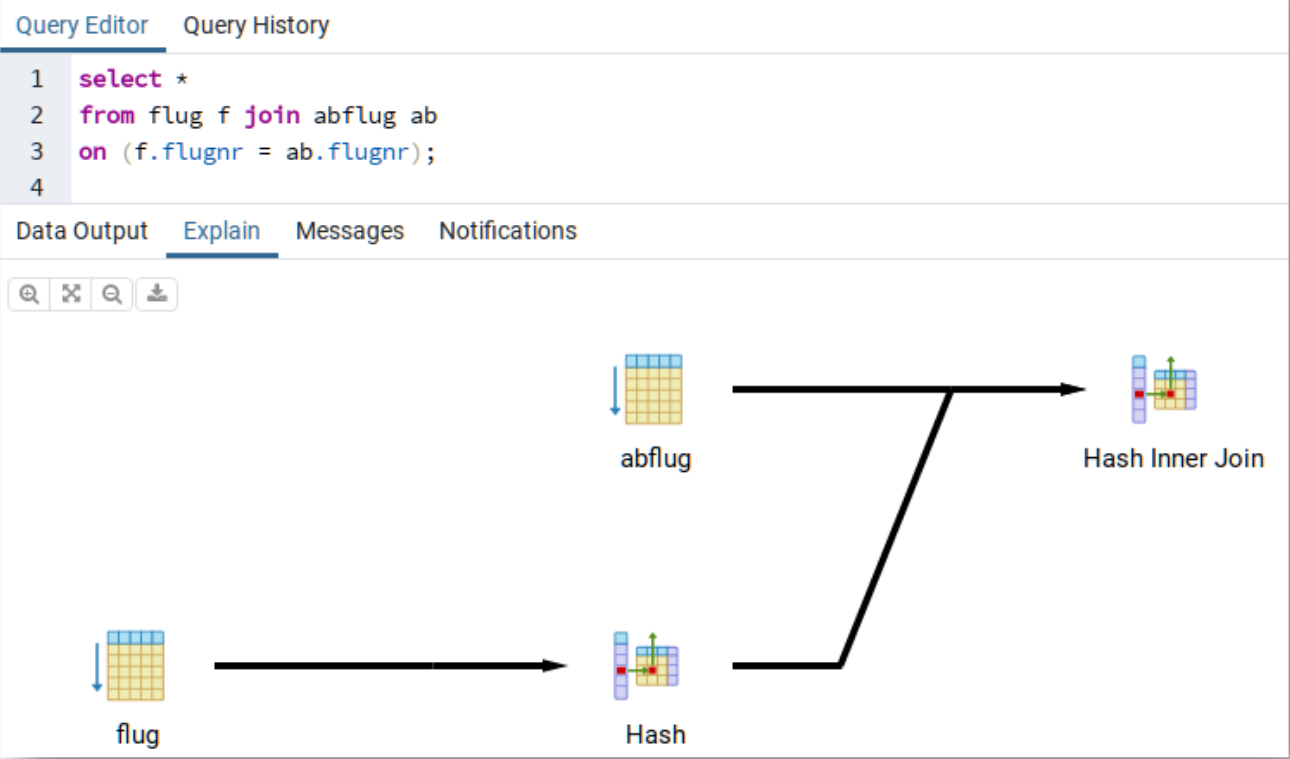
\includegraphics[height=150px]{Explain-Select.png}

Man kann das DBMS auch anweisen, anzuzeigen welchen Ausführungsplan es für eine bestimmte Query benutzen würde. Die Syntax ist hierfür:
\begin{lstlisting}[language=SQL]
    EXPLAIN SELECT ...
\end{lstlisting}

Viele DB-Clients können den Ausführungsplan auch grafisch anzeigen. Im oberen Bild sehen wir ein Beispiel davon für pgAdmin.

\end{document}
